\ifx\preampleIncluded\undefined
\def\startGoedel{}
\documentclass[12pt,a4paper,danish,twoside,reqno]{unf-compendium}

\usepackage[utf8]{inputenc}
\usepackage[danish]{babel}

\usepackage{amsmath, amsthm, amsfonts, amssymb}
\usepackage{bussproofs}
\usepackage{boxproof}
\usepackage{environ}
\usepackage{wasysym}
\usepackage{cleveref}
%\newtheorem{thm}{S{\ae}tning}
%\newtheorem{lem}{Lemma}
%\newtheorem{cor}{Korollar}

\theoremstyle{definition}
\newtheorem{dfn}{Definition}

\theoremstyle{remark}
\newtheorem{eks}{Eksempel}
\renewcommand{\phi}{\varphi}

\newcommand{\nats}{\ensuremath{\mathbb{N}}}
\newcommand{\reals}{\ensuremath{\mathbb{R}}}
\newcommand{\integers}{\ensuremath{\mathbb{Z}}}

\newcommand{\dx}{\,\mathrm{d} x}
\newcommand{\dz}{\,\mathrm{d} z}

\newcommand{\Uline}[1]{\underline{\underline{#1}}}
\newcommand{\vdashv}{\dashv\vdash}
\renewcommand{\imp}{\Rightarrow}
\newcommand{\bimp}{\Leftrightarrow}
\newcommand{\andL}{\wedge}
\newcommand{\orL}{\vee}
%\newcommand{\abs}[1]{\left|#1\right|}

\DeclareMathOperator{\Pfar}{far}
\DeclareMathOperator{\Pmor}{mor}
\DeclareMathOperator{\Pforaelder}{forælder}
\DeclareMathOperator{\Psoeskende}{søskende}
\DeclareMathOperator{\Phs}{hs}
\DeclareMathOperator{\Pfarmor}{farmor}
\DeclareMathOperator{\Pbedstemor}{bedstemor}
\DeclareMathOperator{\Pbedsteforaelder}{bedsteforælder}

\DeclareMathOperator{\Pvfu}{vfu}
\DeclareMathOperator{\pct}{\%}
\DeclareMathOperator{\BevisPar}{BevisPar}
\DeclareMathOperator{\Sub}{Sub}
\DeclareMathOperator{\Quine}{Quine}

\newif\ifsolution
\NewEnviron{solution}{\ifsolution{\par\noindent\textbf{Løsning.} }\expandafter\BODY\hfill$\square$\par\fi}
\theoremstyle{definition}\newtheorem{exercise}{Opgave}

\def\preampleIncluded{}

\begin{document}
\fi

\section{Gödels ufuldstændigheds sætninger}
\subsection{Fuldstændighed og Konsistens}
Lad os betragte en simpel sætning i prædikatlogik (uden Peanos postulater):
\begin{equation}\label{exists-is-forall}
	\vdash \exists x \phi \imp \forall x \phi
\end{equation}
Er det en sand eller falsk sætning? Umiddelbart lyder påstanden "hvis der eksisterer en ting så noget gælder, så gælder det også for alle af den ting" som noget værre vås.
Så det ville nok være oplagt at tro at det er falsk - dvs. at det negerede udsagn er sandt.
Men har vi information nok i vores regler fra prædikatlogik til at afgøre dette? Hvad hvis der kun findes en eneste ting? Det kan vi formulere som
\[
	\vdash \forall x_1 \forall x_2 (x_1 = x_2).
\]
Altså hvis vi tager to ting så er de to ting ens. Lad os se hvad der sker:
\begin{proofbox}
	\lbl{imp_box}
	\[
		\lbl{premise} \\
		\: \exists x \phi \= \text{Antagelse} \\
		\lbl{forall_box}
		\[
			x_0 \= \text{(Lad $x_0$ være givet)} \\
			\lbl{exists_box}
			\[
				\lbl{_1}
				x_\exists \: \phi[x_\exists/x] \= \text{(Start $\exists x$ e \ref{premise})} \\
				\lbl{_ax}
				\: \forall x_1 \forall x_2 (x_1 = x_2) \= \text{Aksiom} \\
				\lbl{_3}
				\: \forall x_2 (x_\exists = x_2) \= \text{$\forall x$ e \ref{_ax}} \\
				\lbl{_4}
				\: x_\exists = x_0 \= \text{$\forall x$ e \ref{_3}} \\
				\label{exists_box_9101b3dded5f472d9c092366392932b2}
				\: \phi[x_0/x] \= \text{$=e$ \ref{_4},\ref{_1}}
			\]
			\label{forall_box_9101b3dded5f472d9c092366392932b2}
			\: \phi[x_0/x] \= \text{$\exists x$ e \ref{exists_box}-\ref{exists_box_9101b3dded5f472d9c092366392932b2}}
		\]
		\label{imp_box_9101b3dded5f472d9c092366392932b2}
		\: \forall x\, \phi \= \text{$\forall x$ i \ref{forall_box}-\ref{forall_box_9101b3dded5f472d9c092366392932b2}}
	\]
	\: \exists x \phi \imp \forall x\, \phi \= \text{$\imp$i \ref{imp_box}-\ref{imp_box_9101b3dded5f472d9c092366392932b2}}
\end{proofbox}
Okay, det var måske ikke så overraskende. Hvis der kun findes en enkelt ting er det ligemeget om noget vi siger at der eksisterere en ting så noget gælder,
eller vi siger noget gælder for alle ting. Hvad sker der hvis vi antager det negerede -- altså at der findes mindst to forskellige ting?
Dvs. vi tilføjer i stedet aksiomet
\begin{equation}\label{exists-isnt-forall}
	\vdash \neg(\forall x_1 \forall x_2 (x_1 = x_2)).
\end{equation}
%Så vi kommer med et bud på et prædikat $\phi$ hvor \eqref{exists-is-forall} går galt.
Hvis vi har mere end en ting så passer det at der for en ting $t_1$ findes en ting $t_2$ så $t_1=t_2$ (dvs. den samme ting findes åbentlyst).
Men det passer ikke at for en ting $t_1$ er alle ting $t_2$ lig med den (da vi jo har et aksiom om at der er mere end en ting!).
%df8a2e0a45d84daba307ea974513a733
\begin{proofbox}
	\lbl{neg_box}
	\[
		\lbl{ass}
		\: \exists x \phi \imp \forall x \phi \= \text{Antagelse} \\
		\lbl{axiom}
		\: \neg(\forall x_1 \forall x_2 (x_1 = x_2)) \= \text{Aksiom} \\
		\lbl{ex1}
		\: \exists x_1 \neg\forall x_2 (x_1=x_2) \= \text{$\forall$ og $\neg\exists$ ækvivalens} \\
		\lbl{eb1}
		\[
			t_1 \: \neg\forall x_2 (t_1=x_2) \= \text{(start $\exists x_1$ e)} \\
			\lbl{ex2}
			\: \exists x_2 \neg(t_1=x_2) \= \text{$\neg\forall$ og $\exists$ ækvivalens} \\
			\lbl{eb2}
			\[
				\lbl{_0}
				t_2 \: \neg(t_1=t_2) \= \text{(start $\exists x_2$ e)} \\
				\lbl{_1}
				\: t_2=t_2 \= \text{$=$i} \\
				\lbl{_2}
				\: \exists x (x=t_2) \= \text{$\exists x$ i \ref{_1}} \\
				\lbl{_3}
				\: \exists x (x=t_2) \imp \forall x (x=t_2) \= \text{Erstat prædikat i \ref{ass}} \\
				\lbl{_4}
				\: \forall x (x=t_2) \= \text{$\imp$e \ref{_3},\ref{_2}} \\
				\lbl{_5}
				\: t_1=t_2 \= \text{$\forall e$ \ref{_4}} \\
				\label{eb2_df8a2e0a45d84daba307ea974513a73}
				\: \bot \= \text{$\neg$e \ref{_5},\ref{_0}}
			\]
			\label{eb1_df8a2e0a45d84daba307ea974513a73}
			\: \bot \= \text{$\exists x_2$ e \ref{ex2},\ref{eb2}-\ref{eb2_df8a2e0a45d84daba307ea974513a73}}
		\]
		\label{neg_box_df8a2e0a45d84daba307ea974513a733}
		\: \bot \= \text{$\exists x_1$ e \ref{ex1},\ref{eb1}-\ref{eb1_df8a2e0a45d84daba307ea974513a73}}
	\]i
	\: \neg(\exists x \phi \imp \forall x \phi) \= \text{$\neg$i \ref{neg_box},\ref{neg_box_df8a2e0a45d84daba307ea974513a733}} \\
\end{proofbox}

Så vi har tilsyneladende en sætning her i prædikatlogik som hverken er sand eller falsk uden at vi tilføjer nogen flere aksiomer.
Vi betegner sådan en sætning som en "ufuldstændighed"{},
og et system der inderholder en ufuldstændighed siges at være et ufulstændigt system.
Hvis et system ikke er ufuldstændigt siges det at være fuldstændigt.
Vi skal bemærke her at selvom vi ikke kan tillægge en sandhedsværdi til sætningen er udsagnet
\[
	\vdash (\exists x \phi \imp \forall \phi) \lor \neg(\exists x \phi \imp \forall \phi)
\]
ikke desto mindre sandt på grund af loven om den udelukkede midte.

Så ved at tilføje et nyt aksiom får vi flere sætninger som vi kan afgøre sandheden af. Det gør altså systemet "stærkere".
Men hvad nu hvis man allerede kunne vise \eqref{exists-isnt-forall} udelukkende med ren prædikatlogik?
Kan vi nu være helt sikre på at der ikke f.eks. er nogen af vores aksiomer der allerede indirekte får der til at være mindst
to elementer? Hvad ville der ske hvis det var tilfældet at vi allerede kunne vise resultatet ovenfor, og vi så tilføjede
\eqref{exists-is-forall} som aksiom? Lad os se hvad der sker:
\begin{proofbox}
	\lbl{_1}
	\: \neg(\exists x \phi \imp \forall x \phi) \= \text{Ting vi kan vise i vores system} \\
	\lbl{_2}
	\: \exists x \phi \imp \forall x \phi \= \text{Aksiom} \\
	\lbl{_3}
	\: \bot \= \text{$\neg$e \ref{_2},\ref{_1}} \\
	\: \psi \= \text{$\bot$e \ref{_3}}
\end{proofbox}
Hov... $\psi$ her kan være hvilket som helst udsagn. Så nu er \text{alt} ligepludselig blevet sandt -- dvs. alle sætninger inkl. deres negerede,
så alt er både sandt og falsk på samme tid. Det der skete her er hvad man på engelsk betegner "Principle of Explosion"{}. Hvis man kommer frem til en
modstrid uden nogen antagelser (uden for en boks og uden præmisser), så falder hele systemet fra hinanden. Eller som xkcd forklarer det:
\\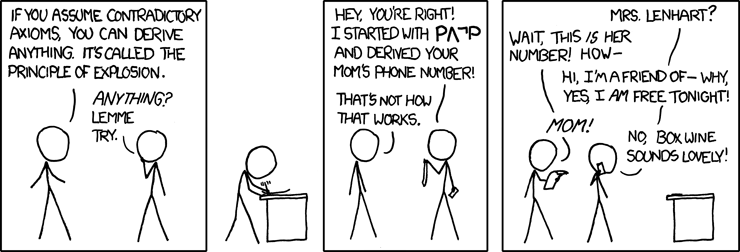
\includegraphics[width=\textwidth]{principle_of_explosion.png}

Hvis et logisk system falder sammen på sådan en måde siger vi at det er inkonsistent --
kombinationen af de modstridende aksiomer danner tilsammen en inkonsistens.
Hvis et system ikke er inkonsistent siger vi at det er konsistent.
Inkonsistente systemer er af åbentlyse grunde ret uinteressante.
Men det kan hurtigt blive svært at formulere et sæt aksiomer der beskriver komplicerede ting
og stadigvæk være sikker på at der ikke er nogen ting der strider mod hinanden.
Da man forsøgte at bygge matematikken op fra et grundlag af formel logik i slutningen
af 1800-tallet til starten af 1900-tallet stødte man flere gange ind i sådan nogen problemer,
hvor nogen nok specielt har hørt om Rusells Paradoks -- dette vil vi dog ikke komme nærmere
ind på her.

Så vi har altså to forskellige egenskaber som logiske systemer kan have: Fuldstændigt og Konsistent.
Optimalt set ville det jo være rart hvis et system er begge dele.
Men kan vi få det til at være dette? Og kan vi analysere om et system har de egenskaber?
Det første spørgsmål man kunne stille ville være hvad man ville analysere systemet med. Hvordan kan vi vide at det
vi bruger til at analysere systemet med selv er konsistent? Hvis det ikke er så ville det jo også kunne fortælle
os at systemet er inkonsistent, og så kan vi ikke rigtigt sige at være kommet frem til noget.
En ting man kunne håbe på kunne jo være at man kunne bruge et tilsyneladende simplere system til at analysere et mere komplekst system.
Selvom vi ikke ville vide det med sikkerhed kan vi måske føle os mere sikre på at et simplere system er konsistent.

Nogen systemer er så simple at vi nemt kan analysere dem. F.eks. kan vi vise at ren udsagnslogik er både fuldstændigt og konsistent.
Årsagen til dette er at man kan analysere den fulde opførsel af $\land,\lor,\imp,\neg$ og $\bimp$ ved at skrive endelige sandhedstabeller op som man
kan kontrollere værdien/korrektheden af. Lige så snart vi har med prædikatlogik at gøre kan man sådan lidt uformelt sige at vi
har introduceret et potentiale for uendelighed, så vi har ikke længere noget hvor vi kan analysere et endeligt antal muligheder.

Så kan vi så analysere prædikatlogik på en anden måde? Det kunne jo være meget rart at vide med rimelig sikkerhed om 
f.eks. \eqref{exists-is-forall} er en ufuldstændighed. Svaret er at det er det -- vi kan bl.a. angribe problemet med
noget der hedder modelteori (som forøvrigt forvirrende nok har sit eget fuldstændighedsbegreb). Beviser der snakker
om logiske systemer betegner vi som metabeviser -- det er metalogik når man analysere logiske systemer.

Vi vil dog ikke komme nærmere ind på modelteori her.
Hvad vi vil komme ind på er hvordan man kan formalisere beviser om logiske systemer så de selv kan beskrives
af logiske systemer. Det viser sig at man på den måde kan få nogen stærke sætningner om hvad vi kan vise
om systemers fuldstændighed og konsistens.

\subsection{$\omega$-inkonsistens og $\omega$-ufuldstændighed}
Vi så på hvordan systemer der ikke har stærke nok aksiomer bliver ufuldstændige.
Et godt spørgsmål kunne jo være om f.eks. peanoaritmitikken (herfra betegnet P.A.)
er fuldstændig. Lad os starte med at se på hvad der sker hvis vi fjerne induktionsaksiomet.
Vi så hvordan vi viste at $0+a=a$ ved at bruge induktion. Uden induktionsaksiomet kan vi
f.eks. vise $0+S(0) = S(0)$ -- altså $0+1=1$ -- ved at følge hvad der bliver
gjort inde i den inderste af boksene i beviset hvor vi erstatter $a_0$ med $0$.
Når vi har vist dette kan vi gøre det samme med $0+S(S(0)) = S(S(0))$ osv.

Altså kan vi vise sætningerne
\begin{flalign*}
	0+0 &= 0 \\
	0+S(0) &= S(0) \\
	0+S(S(0)) &= S(S(0)) \\
	0+S(S(S(0))) &= S(S(S(0))) \\
	&\vdots
\end{flalign*}

Ikke desto mindre er vi ude af stand til at vise den generelle sætning
\[
	\forall a \, a+a=a
\]
uden induktionsaksiomet. Vi kalder sådan en ufuldstændighed for en $\omega$-ufuldstændighed.
For at præcisere det: \textit{En $\omega$-ufuldstændighed er en ubeviselig sætning der omhandler noget der gælder for alle objekter men hvor vi kan bevise sætningen for hvert enkelt element når det er eksplicit givet.}

Hvad sker der hvis nu vi i stedet for at tilføje induktionsaksiomet så vælger at tilføje den
negerede af den generelle sætning? Altså vi tilføjer som aksiom
\[
	\neg\forall a \, a+a=a
\]
hvilket er ækvivalent med $\exists a \, \neg(a+a=a)$. Vi kan stadigvæk vise sætningerne for hvert enkelt tal er sande, men nu har vi ligepludseligt fået nogen mærkelige tal der opfører sig anderledes. Vi kalder denne situation for en $\omega$-inkonsistens.
\textit{En $\omega$-inkonsistens er en sand sætning der omhandler noget der gælder for alle objekter men hvor vi kan bevise den negerede sætning for hvert enkelt element når det er eksplicit givet.}

Sådan en $\omega$-inkonsistens virker nok som en lidt spøjs ting, men det er langt fra så slemt som en rigtig inkonsistens. Det får ikke på nogen måde systemet til at falde fra hinanden.
Faktisk er der velkendte sætninger i matematik der er eksempler på $\omega$-inkonsistenser -- f.eks. Banach-Tarski paradokset er af en sådan natur.

\subsection{Metasætninger i P.A}
Det viser sig at vi er i stand til at vise ting om et vilkårligt logisk system udelukkende ved
brug af Peanos aksiomer. Men de taler kun om tal, så hvordan søren kan vi pludselig få dem
til at omtale udsagn og beviser?
Tricket beror på hvad der kaldes Gödel nummerering. Vi kan tage hvert tegn vi bruger i
logik og tildele et tal. F.eks. til at beskrive udsagnslogik kunne vi definere
\begin{align*}
	\phi:& 01 &
	\psi:& 02 \\
	\chi:& 03 &
	\alpha:& 04 \\
	\{\,:& 10 &
	\}:& 11 \\
	\imp:& 12 &
	\bimp:& 13 \\
	\land:& 14 &
	\lor:& 15 \\
	\neg:& 16 &
	\bot:& 17 \\
	(\,:& 18 &
	):& 19
\end{align*}
Vi bruger her \{ og \} til at indikere start og slut på bokse.
Vi kan selvfølgelig udvide oversættelsen med flere tegn som f.eks. dem vi skal bruge
i prædikatlogik og peanoaritmetik. Ligeledes kan vi tilføje flere udsagnsplaceholders og
variable etc. Vi kan nu tage et udsagn i udsangslogik og oversætte med vores definitioner:
\[
	\underset{01}{\phi} \underset{14}{\land\vphantom{\phi}} \underset{02}{\psi} \underset{12}{\imp\vphantom{\phi}}
	\underset{02}{\psi} \underset{14}{\land\vphantom{\phi}} \underset{01}{\phi}
\]
Tallet 01140212021401 her er hvad vi kalder for udsagnets Gödel nummer -- eller forkortet G.n.
Vi vil referere til et udsagns Gödel nummer ved at puttet udsagnet i mellem $\langle$ og $\rangle$ tegn. F.eks.
\[
	\langle \phi \land \psi \imp \psi \land \phi \rangle = 01140212021401
\]

Vi er nu i stand til at skriver sætningner op i P.A. der omhandler andre sætninger.
Vi vil ikke gå i detaljer med præcist hvordan det gøres, men demonstrere et eksempel
på en af egenskaberne for at gøre den generelle idé klar. Vi vil her bruge division
til at indikere heltals division og definere $\%$ som divisionsrest.
Altså betyder $a\pct b$ resten efter at dividere $a$ med $b$.
Den første egenskab vi skal bruge er velformethed.
Det vil sige om et udsagn overhovedet giver mening -- f.eks. er $\phi)\land\lor$ et ugyldigt udsagn.
Vi betegner denne egenskab ved prædikatet $\Pvfu(n)$, hvor "vfu"{} står for "VelFormet Udtryk".

Vi kunne forestille os at $\Pvfu(n)$ havde en definition der så ud som noget i retning af
\begin{flalign*}
	\Pvfu(n) := \Pvfu_\imp(n) \lor (\neg\Pvfu_\imp(n) \land \Pvfu_\land) \lor \ldots \lor \Pvfu_u(n)
\end{flalign*}
hvor
\[
	\Pvfu_\imp(n) := \exists m \left(
		\frac{n}{10^{2m}} \pct 100 = 12 
		\land \Pvfu\left(n\pct 10^{2m}
		\land\Pvfu\left(\frac{n}{10^{2m+2}}\right)\right) \right)
\]
og
\[
	\Pvfu_u(n) := n \geq 1 \land n \leq 4
\]

Følgende skulle gerne demonstrere idéen bag:
\[
	\underbrace{\underset{01}{\phi} \underset{14}{\land\vphantom{\phi}} \underset{02}{\psi}}_{\frac{n}{10^{2m+2}}}
	\underbrace{\underset{12}{\imp\vphantom{\phi}}}_{\frac{n}{10^{2m}} \pct 100}
	\underbrace{\underset{02}{\psi} \underset{14}{\land\vphantom{\phi}} \underset{01}{\phi}}_{n\pct 10^{2m}}
\]

Vi vil ikke pensle ud hvordan reglerne for alle tegnene skal opbygges her. Det afgørende at bemærke her er at vi
helt slavisk kan kontrollere om prædikatet er opfyldt. Vi kan, givet Gödel tallet for et vilkårligt udsagn, konstruere
et bevis for om det er velformet eller ej. I princippet skal vi bare tjekke hver af kravene igennem og tjekke det
endelige antal muligheder for $m$ igennem. Hver af kravene der selv referere til prædikatet deler det op i mindre
bider, så vi er garanteret at vi med et endelig antal trin kan kontrollere hele udsagnet.

Ligesom vi kan definere et prædikat der siger om et tal er G.n. for et velformet udsagn kan vi også definere et der siger
siger om et talpar udgør en sætning med et bevis herfor:
\[
	\BevisPar(b,u):= \text{$b$ er et gyldigt bevis for udsagnet $u$}
\]
Så vi kan f.eks. skrive
\[
	\exists b \BevisPar(b,u_0)
\]
Som betyder: "Der findes et bevis med G.n. $b$ for udsagnet med G.n. $u_0$".

\subsection{Gödels første ufuldstændighedsætning}
Vi vil nu til at prøve at konstruere et udsagn der siger "Jeg kan ikke bevises i P.A."{}. Det er nok ikke helt åbentlyst at
et sådan udsagn overhovedet kan konstrueres. Man hvis det kan har vi et udsagn der må være en ufuldstændighed i P.A.
da den er et eksempel på løgnerparadokset så den hverken kan være sand eller falsk.

Den første idé her er at definere et nyt prædikat:\\
$\Sub(u,a,u'):= $ $u'$ er G.n. for sætningen med G.n. $u$ hvor en fri variabel er blevet erstattet med $a$.

Altså prædikatet udtaler sig om hvorvidt en sætning tilsvarer en anden sætning hvor vi har erstattet en fri variabel med en bestemt værdi.
Man kan eksplicit definere sådan en operation ved at sætte en masse aritmetiske/talteoretiske operationer sammen der operere på 10'er potenser.
Vi har igen ikke tænkt os at pensle det ud, vi vil bare bemærke at det er en operation hvis uden problemer skulle kunne udføre
i hånden og som kan beskrives i P.A. Det interessante er hvad der sker hvis $u=a$.
Vi giver også dette tilfælde et navn:
\[
	\Quine(u,u') := \Sub(u,u,u')
\]

Vi kan formulere $\Quine(u,u')$ som: $u'$ er G.n. for udsagnet med G.n $u$ hvor en fri variabel er erstattet med $u$. Med andre ord så erklærer prædikatet at vi har lavet en ny sætning ved at erstattet en fri variabel med Gödel nummeret for den gamle sætning. F.eks. er
\[
	\Quine(\langle x=S0 \rangle, \langle\langle x=S0\rangle=S0\rangle)
\]
sand. Sætningen $\langle x=S0 \rangle = S0$ er selvfølgelig falsk.

Vi definerer nu et udsagn der benytter sig af dette
\[
	G_0 := \neg\exists b \exists u \left( \BevisPar(b,u) \land \Quine(u_0,u) \right)
\]
Den siger: "Der findes ikke en sætning med G.n. $u$ så $u$ er $u_0$ hvor en fri variabel er erstattet med $u_0$".

Det interessante er nu hvad der sker hvis vi prøver at indsætte dens eget Gödel nummer for $u_0$.
Vi ser på udsagnet
\[
	G := \neg\exists b \exists u \left( \BevisPar(b,u) \land \Quine(\langle G_0 \rangle,u) \right)
\]
Hvad siger det så? "Der findes ikke en sætning med G.n. $u$ så $u$ er G.n. for $G_0$ hvor
$u_0$ er erstattet med G.n for $G_0$". Så hvordan ser $G_0$ så ud når vi er erstatter $u_0$ med $\langle G_0 \rangle$?
\[
	G_0[\langle G_0 \rangle/u_0] := \neg\exists b \exists u \left( \BevisPar(b,u) \land \Quine(\langle G_0 \rangle,u) \right)
\]
Men det var jo netop $G$. Så vores $u$ er altså G.n for $G$ selv. Nu er $G_0$ jo et udsagn som vi ved findes og som kan
vi kan finde Gödel nummeret på samt erstatte den frie variable $u_0$ med dette tal på.
Altså må udsagnet $u$ eksistere. Så årsagen til at sætningen er falsk må være at $b$ ikke findes -- altså at $u$ ikke er en sætning.

Men så må det G siger være: "Der findes ikke noget bevis for udsagnet med G.n. $u$".
Eller med andre ord "$G$ kan ikke bevises i P.A.". Som nævnt før må dette betyde at hvis vi kan vise $G$ har vi en modstrid.
Samtidig hvis vi kan vise $\neg G$ så siger $\neg G$: "$G$ kan bevises i P.A.", hvilket igen er en modstrid.
Vi kan altså konkludere at $G$ er en ufuldstændighed i P.A. Faktisk kan vi vise at der er tale om en $\omega$-ufuldstændighed.
Betragt nemlig
\[
	\forall b \neg \exists u (\BevisPar(b,u) \land \Quine(\langle G_0 \rangle, u))
\]

Det udsagn kan ikke udgøre en sætning i P.A. For ellers kunne vi bruge $\forall b$ e til at bevise $\neg G$. Men da $G$ jo ikke er en sætning
kan der omvendt heller ikke eksistere noget $b$ så $b$ er et bevis for $G$. Ethvert tal vi måtte sætte ind på $b$s plads vi derfor give
os en sand sætning (altså som vi kan bevise). Så hvad ville der så ske hvis vi indførte ovenstående som et aksiom?
Nu ville vi have et nyt $\BevisPar$ prædikat eftersom hvilke beviser der er gyldige afhænger af hvilke aksiomer der er i systemet.
Derfor får det nye system også en ny $G$ som er en ufuldstændighed. Det skulle være klart at vi altid vil støde ind i det problem
uanset hvilke aksiomer vi har sålænge man kan arbejde med Peano aritmitik i systemet.

\subsection{Gödels anden ufuldstændighedssætning}
Hvis vi virkeligt gad gøre arbejdet og udpensle alt i sidste bevis til mindste detalje kunne vi skrive det op som et formelt bevis i logik.
Dette bevis kan naturligvis selv kodes som et Gödel nummer.
Lad os nu antage at vores logiske system er konsistent og vi har et bevis for dette.
I såfald vil der eksistere et bevis for at $G$ ikke er en sætning i systemet.
Men det vil sige at $\neg G$ er en sætning hvilket førte til en modstrid.
Så vi må konkludere at et system der kan beskrive P.A. er ude af stand til at indeholde en sætning om sin egen konsistens medmindre det er inkonsistent.

\ifdefined\startGoedel\end{document}\fi
